\documentclass[12pt,a4paper,oneside]{book}
\usepackage[utf8]{inputenc}
\usepackage[spanish]{babel}
\usepackage[toc,page]{appendix}
\usepackage{longtable}
\usepackage{amsmath}
\usepackage{amsfonts}
\usepackage{amssymb}
\usepackage{listingsutf8}
\usepackage{color, soul}
\usepackage{paracol}
\usepackage{lipsum}


%%%%%%%%%%%%% Macros para formato 302 %%%%%%%%%%%%%%%%%%%

% Metadata para el PDF a generar 
\usepackage[unicode,
            pdftex]{hyperref}
\hypersetup{
 pdfauthor={PONER LOS NOMBRES DE LOS AUTORES},
 pdftitle={PONER EL TITULO},
 pdfsubject={PONER EL SUBTITULO},
 pdfkeywords={PONER PALABRAS CLAVE}
 }

% Numeración y formato de páginas
\usepackage{fancyhdr}
\pagestyle{fancy}
\fancyhf{}
%\fancyhead[lo,le]{\nouppercase{\rightmark}}
\fancyfoot[RO]{\thepage}

\fancypagestyle{plain}{
  \fancyhf{} 
  \fancyfoot[RO]{\thepage}
  \renewcommand{\headrulewidth}{0pt}}
\renewcommand{\headrulewidth}{0pt}


% Indice (estos parámetros se pueden cambiar)
\setcounter{secnumdepth}{3} %para que ponga 1.1.1.1 en subsubsecciones
\setcounter{tocdepth}{3} % para que ponga subsubsecciones en el indice

%% Para incluir imagenes
\usepackage{graphicx}


% Para incluir tablas en español
\renewcommand\tablename{\bfseries Tabla}

% Para incluir listings de código
\renewcommand{\lstlistingname}{\bfseries C\'odigo}

% Para agregar la bibliografía al indice
\usepackage[nottoc,numbib]{tocbibind}


%%%%%%%%%%%%%%%%%%%%%%%%%%%%%%%%%%%%%%%%%%%%%%%%%%%%%%

% Generación del índice
\makeindex

% Empieza el documento
\begin{document}

% Portada (completar con los datos)
\vspace*{\fill}

\begin{center}

\begin{Large}
\textbf{Universidad ORT Uruguay}

\textbf{Facultad de Ingeniería}
\vspace{5cm}
\end{Large}

\begin{huge}
\textbf{Título del trabajo}
\end{huge} 

\begin{Large}
Subtítulo (opcional)
\end{Large}
\bigskip
\bigskip


\textbf{Entregado como requisito para la obtención del título de XXX}
\vspace{5cm}

\begin{Large}
\textbf{Nombre Autor 1 - Nro Estud.}\\
\textbf{Nombre Autor 2 - Nro Estud.}\\
\textbf{Nombre Autor 3 - Nro Estud.}\\
\bigskip

\textbf{Tutor: Nombre y Apellido}
\vspace{2cm}
\end{Large}

\begin{huge}
\textbf{2017}
\end{huge}

\end{center}
\vspace*{\fill}

\thispagestyle{empty}
\newpage




\chapter*{Declaración de autoría}


Nosotros, XXX, YYY y ZZZ declaramos que el trabajo que se presenta en esta obra es de nuestra
propia mano. Podemos asegurar que:
\begin{itemize}
\item La obra fue producida en su totalidad mientras realizábamos el Proyecto.
\item Cuando hemos consultado el trabajo publicado por otros, lo hemos atribuido con claridad.
\item Cuando hemos citado obras de otros, hemos indicado las fuentes. Con excepción de estas citas, la obra es enteramente nuestra.
\item En la obra, hemos acusado recibo de las ayudas recibidas.
\item Cuando la obra se basa en trabajo realizado conjuntamente con otros, hemos explicado claramente qué fue contribuido por otros, y qué fue contribuido por nosotros.
\item Ninguna parte de este trabajo ha sido publicada previamente a su entrega, excepto donde se han realizado las aclaraciones correspondientes.
\end{itemize}

 
\vspace{2cm}


\noindent Incluir las firmas escaneadas en el mismo directorio, con los nombres signature1.jpg, signature2.jpg,.. y descomentar las líneas de abajo.\\

%\includegraphics[scale=0.4]{signature1.jpg} \hfill %\includegraphics[scale=0.4]{signature2.jpg} \hfill %\includegraphics[scale=0.4]{signature3.jpg}\\

XXXX \hfill YYYY \hfill ZZZZ\\

fecha \hfill fecha \hfill fecha



\chapter*{Dedicatoria (opcional)}

No es obligatorio incluirla.



\chapter*{Agradecimientos (opcional)}
No es obligatorio incluirlos. Se trata de un breve reconocimiento a personas o instituciones que de diversas maneras han ayudado en la elaboración del trabajo. 
Asegúrese de usar los nombres correctos y completos de las instituciones y las personas que cite aquí.



\chapter*{Abstract}

Consiste de un resumen del contenido del trabajo, que se usa para difusión y para que el lector potencial sepa en qué consiste el trabajo sin necesidad de leerlo completamente. Puede tener una extensión máxima de 400 palabras. Debe existir coherencia entre el contenido del trabajo final y el abstract. Ver documento 306 (Orientación para títulos, resúmenes o abstracts e informes de corrección de trabajos finales de carrera)



\chapter*{Palabras clave}

XXX, YYY, ZZZ


\vspace{1cm}

Conjunto de palabras que están directamente relacionadas con el contenido de la obra que además deberán ser incluidas en las
propiedades del archivo PDF para facilitar que el documento sea indexado por los buscadores.


%el siguiente comando genera el índice (no tocar)
\tableofcontents


\chapter{Introducción} 
\label{intro} % para poder referenciarlo después usando \ref{intro}

A modo de ejemplo introducimos el siguiente texto autogenerado:
\lipsum[1]


Ejemplo de lista utilizando itemize:
\begin{itemize}
    \item Primero
    \item Segundo
    \item Tercero\\
\end{itemize}

Ejemplo de enumeración utilizando enumerate:
\begin{enumerate}
    \item Primero
    \item Segundo
    \item Tercero\\
\end{enumerate}

Ejemplo de enumeración anidada utilizando enumerate:
\begin{enumerate}
    \item Primero 
        \begin{enumerate}
        \item Primero
        \item Segundo
        \item Tercero
        \end{enumerate}
    \item Segundo
        \begin{enumerate}
        \item Primero
            \begin{enumerate}
            \item Primero
            \item Segundo
            \end{enumerate}
        \item Segundo
        \end{enumerate}
\end{enumerate}



\section{Ejemplo de Sección}
\label{secc1}

Para incluir una referencia bibliográfica se utilizará el comando cite:~\cite{girard1989}.
Ejemplo de una cita múltiple:~\cite{ranta2012,tcs2015}.\\

También podemos utilizar el comando ref hacer referencia a una capítulo o sección que haya sido indexada con el comando label. Por ejemplo, la introducción, que es el Capítulo~\ref{intro}, o esta misma sección que es la~\ref{secc1}. Ref también sirve para referenciar figuras, como la Figura~\ref{fig1}, que está más adelante en el texto.



\section{Otra sección}

\lipsum[3]




\subsection{Subsección}

\lipsum[4]


\subsubsection{Subsubsección}

\lipsum[5]

\subsection{Subsección}

\lipsum[6]



\chapter{Otro Capítulo}

Notar quue se genera una página nueva al iniciar un capítulo.

\section{Otra Sección}

En esta sección incluimos una figura.
\begin{figure}[ht]
 \centering
 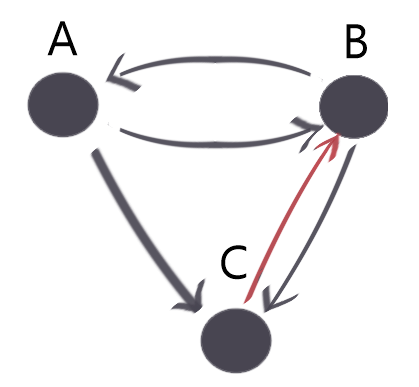
\includegraphics[width=0.5\textwidth]{grafo.png}
 \caption{Figura de ejemplo.}
 \label{fig1}
\end{figure}

\subsection{Otra Subsección}
\lipsum[2-5]

\chapter{Conclusiones}
\lipsum[1-6]




\bibliographystyle{IEEEtran}
%%bibliography
%% No borrar estas dos líneas. Revisar de tener los archivos IEEETran y biblio.bib en la misma carpeta
%% si no están y no anda, correr el compilador de latex varias veces. Primero el bibtex, luego pdflatex, luego pdflatex otra vez.
\bibliography{biblio}


\appendix %A partir de acá los capítulos se enumerarán A, B, C, etc


\chapter{Nombre del Apéndice 1} 
\lipsum[1]
\section{Una Sección}
\lipsum[2-3]
\subsection{Una Subsección}
\lipsum[4-6]

\chapter{Nombre del Apéndice 2} 
\lipsum[6-9]

%\end{appendices}





\end{document}

